\chapter{Basis Functions}
\label{ch:dwt}

%\item Explain MSE, PSNR
In Section \ref{sect:compression}, we introduced transform coding.
We said that any discrete signal $\bm v \in \mathbb{R}^M$ can be expressed in a different basis via a basis transform:
\begin{equation*}
  \bm v = \bm\Psi\bm w
\end{equation*}
where $\bm\Psi$ is the $M\times M$ basis matrix and $\bm w \mathbb{R}^M$ is the representation of $\bm v$ in the $\bm\Psi$ basis.

The particular classes of signals $\bm v$ that we are interested in are digital images and digital video.
The aim of this chapter is to construct a basis matrix $\bm\Psi$ that gives us a (near-) sparse representation of a wide range of such signals $\bm v$.
Finding a set of basis functions $\bs\Psi$ that achieve such a transformation lies at the heart of many lossy compression techniques.

It is important to note here that the choice of basis functions $\bs \Psi$ typically has a significant effect on the performance of the reconstruction algorithms.

\section{Discrete Cosine Transform}
The first basis transform that we will use is the Discrete Cosine Transform (DCT), one of the most widely used transforms in signal processing.
It underlies JPEG image compression and is used in various video compression algorithms such as MJPEG, MPEG, H.261 and H.263 \cite{zeng2013}.
\footnote{A related transform, known as the \emph{Modified DCT} is used in many lossy audio compression formats such as MP3, AAC and Vorbis.}

A DCT decomposes a signal in terms of cosine functions with different frequencies.
Its extensive use in lossy compression algorithms is due to the DCT's \emph{energy compaction} properties.
The majority of a signal's energy is contained within relatively few coefficients - typically those corresponding to the lower frequency basis functions.

On a side note, the DCT comes in a various versions that have minor differences between them.
In the following, we will describe the most widely used version, known as the \emph{DCT-II}, as well as its inverse transform, the \emph{DCT-III}.
We will refer to them simply as ``the DCT'' and ``the Inverse DCT (IDCT)'', respectively.

\subsection{One-Dimensional DCT}
\begin{figure}
  \centering
  \begin{subfigure}{0.45\textwidth}
    \centering
    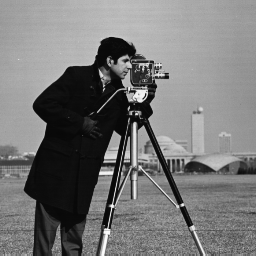
\includegraphics[width=\textwidth]{Chapter3/Images/cameraman.png}
    \caption{Original signal $\bm v$}
  \end{subfigure}
  \begin{subfigure}{0.45\textwidth}
    \centering
    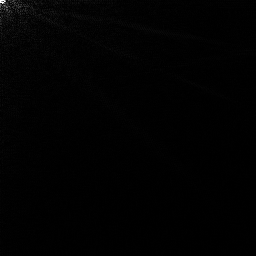
\includegraphics[width=\textwidth]{Chapter3/Images/dctCoeff.png}
    \caption{DCT of $\bm v$}
  \end{subfigure}
  \caption{Panel (a) shows the original signal $\bm v$, a 256$\times$256 grayscale image known as ``cameraman''. Panel (b) illustrates the 2-D DCT of $\bm v$. The brightness of a an element increases with the absolute value of the corresponding DCT coefficient. (The high-frequency coefficients have been enhanced to show more detail).}
  \label{fig:ch3:dct}
\end{figure}

Formally, the DCT $\bm w$ of a one-dimensional signal $\bm v$ of length $M$ is given by
\begin{equation}
  w_k = c(k) \sum_{m=1}^{M} v_m \, \cos\left(\frac{\pi(2i-1)(k-1)}{2M}\right) \qquad k = 1,\cdots,M
\end{equation}
where
\begin{equation*}
  c(k) = \left\{\begin{array}{ll}
  \sqrt{\frac{1}{M}} & \qquad\mbox{if $k=1$}\\
  \sqrt{\frac{2}{M}} & \qquad\mbox{otherwise}\\
  \end{array}\right.
\end{equation*}
This transforms a signal $\bm v$ in the original domain (time or space) into its representation $\bm w$ in the DCT domain.

\begin{figure}
  \centering
  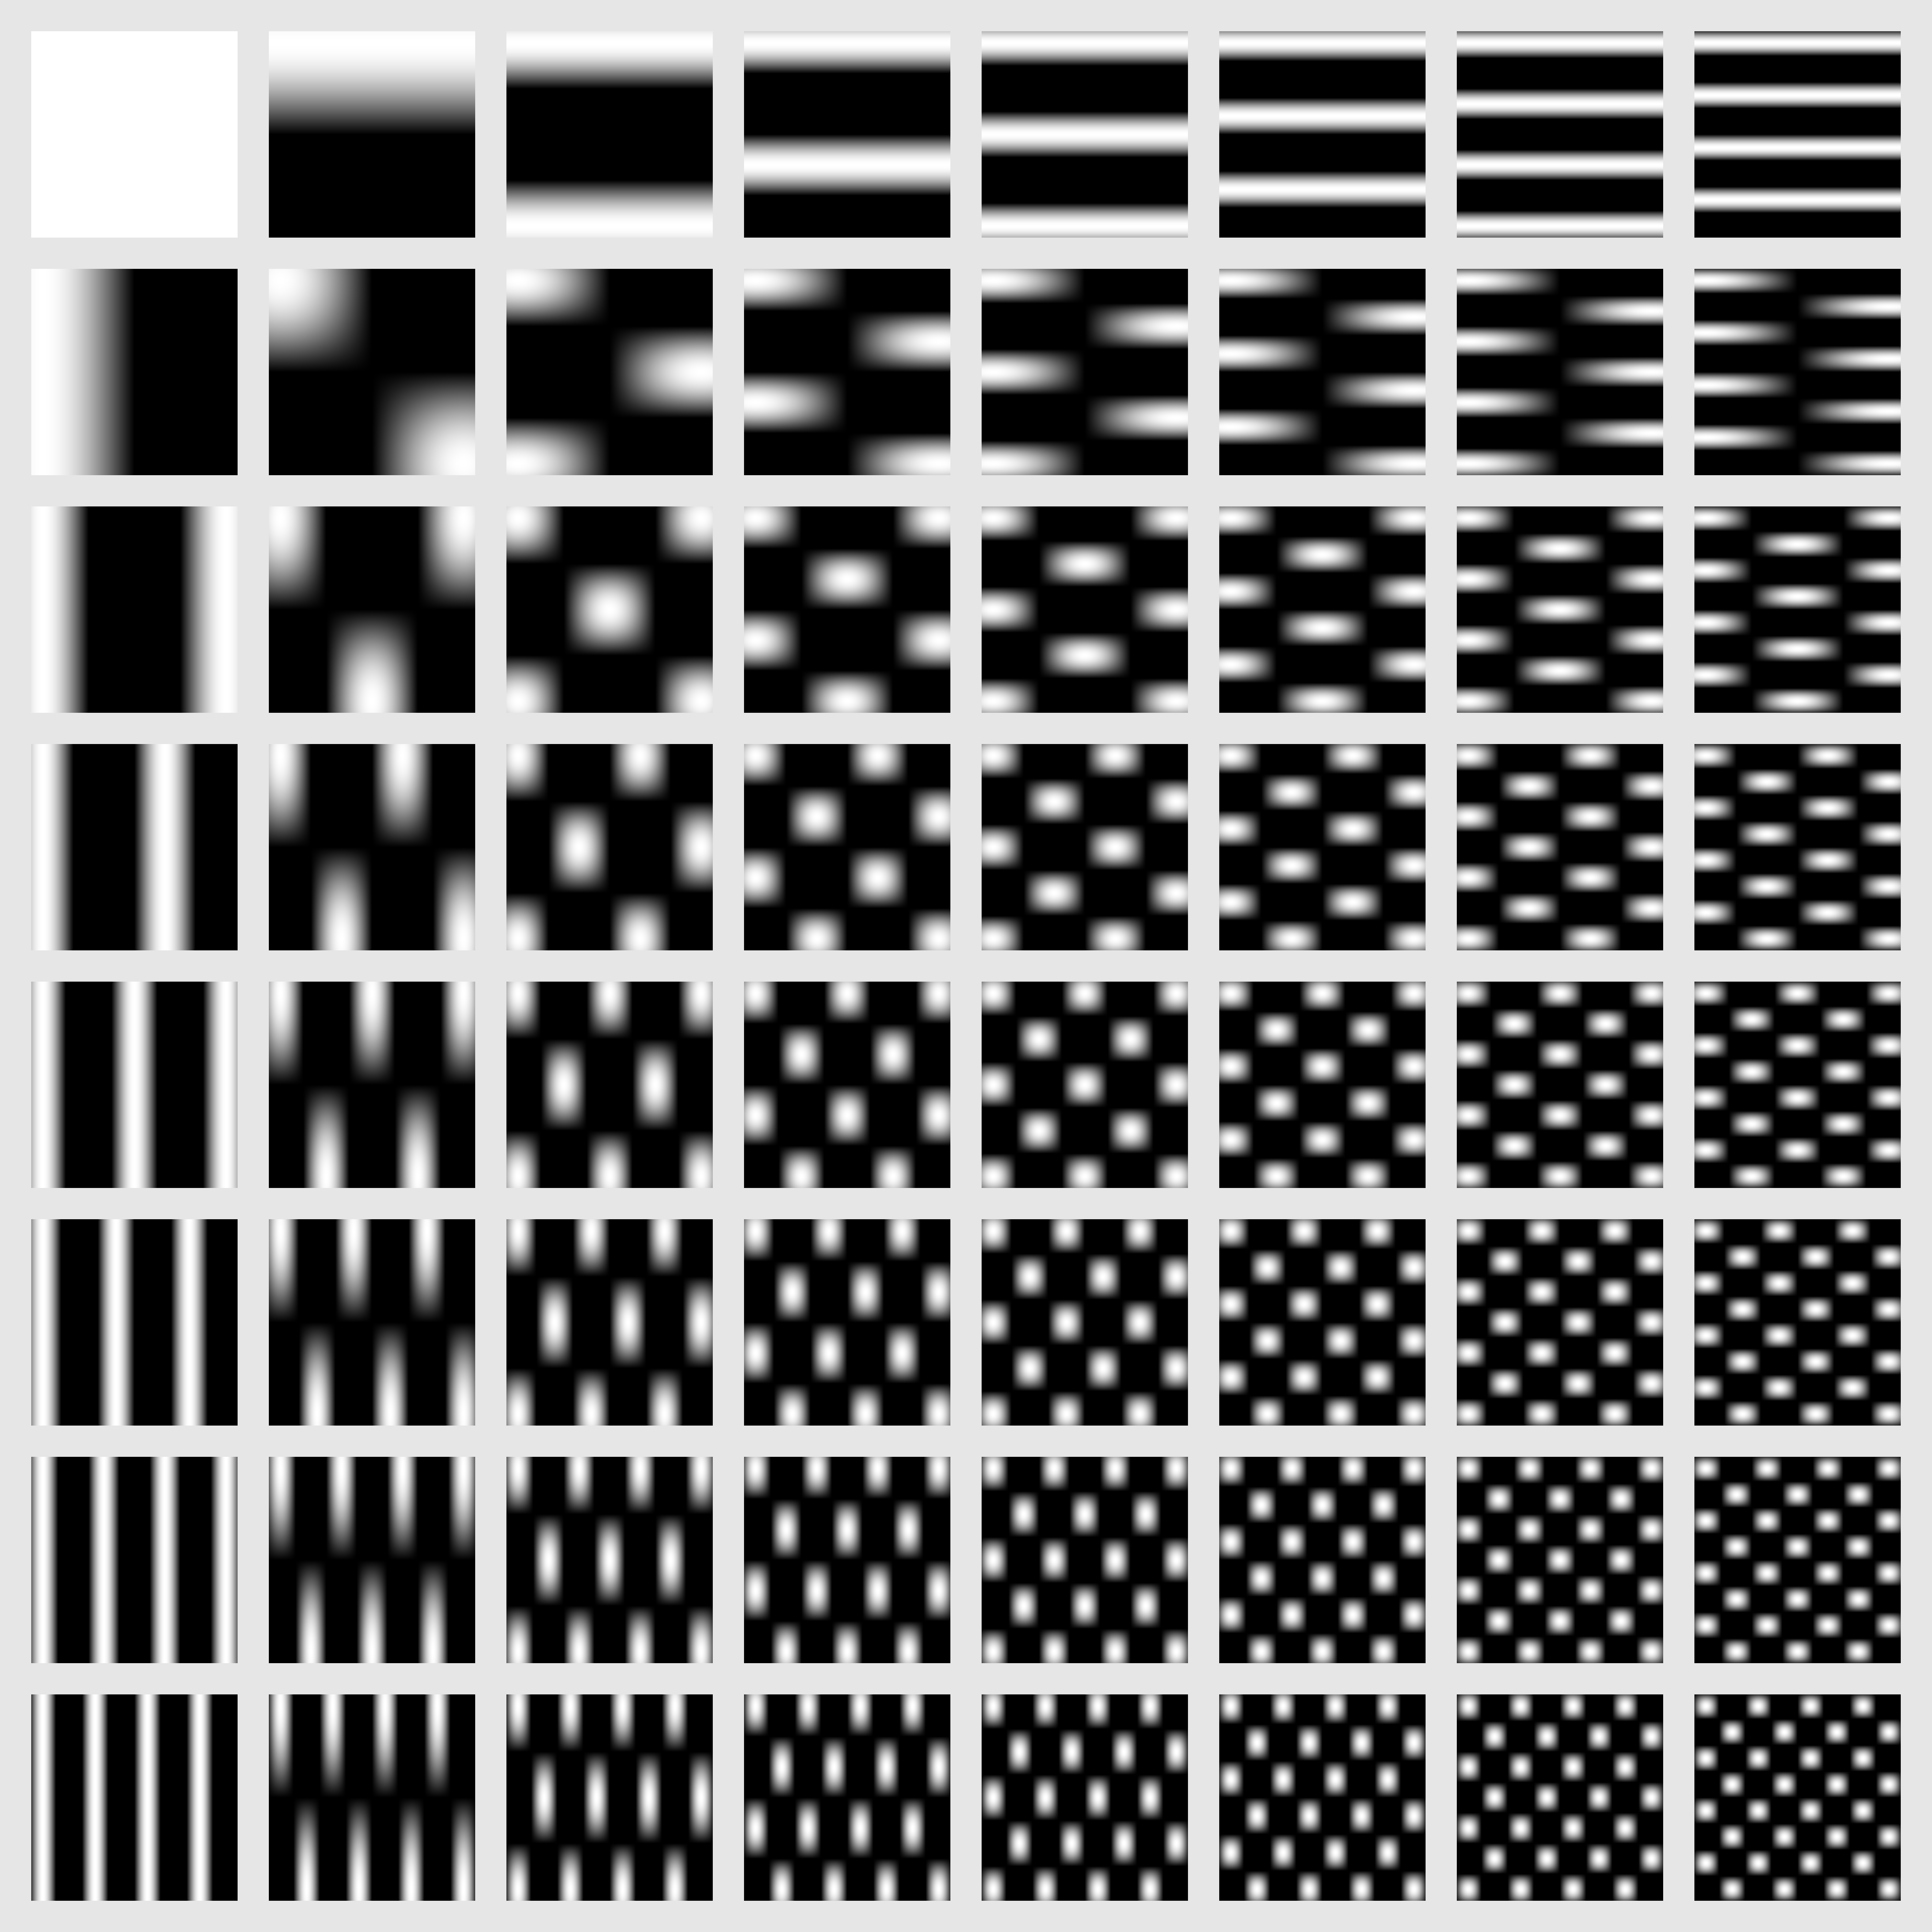
\includegraphics[width=0.5\textwidth]{Chapter3/Images/dct2functions.png}
  \caption{The 2-D DCT basis functions that are used by the DCT to decompose a $8\times 8$ image. 
    The spatial frequency increases towards the bottom right corner.}
  \label{fig:2D-DCT}
\end{figure}

Conversely, given a signal $\bm w$ in the DCT domain, we can transform it back to the orignal (time or space) domain via the IDCT defined by
\begin{equation}
  \label{eqn:idct}
  v_n = \sum_{k=1}^M c(k) w_k  \, \cos\left(\frac{\pi(2i-1)(k-1)}{2M}\right) \qquad n = 1,\cdots,M
\end{equation}

We can express equation (\ref{eqn:idct}) in the desired form $\bm v=\bm P\bm w$.
The entries of the basis matrix $\bm P$ are given by
\begin{equation}
  P_{n,k} = c(k)\, \cos\left(\frac{\pi(2i-1)(k-1)}{2M}\right).
\end{equation}
Note that the basis matrix $\bm P$ is orthogonal, $\bm P^T\bm P=\bm I_M$.

\subsection{Multi-Dimensional DCT}
Once we know how to perform the DCT on a one-dimensional signal, we can easily extend the transform to multi-dimensional signals (images, video, etc).
To do so, we simply perform successive 1-D transforms along each dimension of the signal.
This property is known as \emph{seperability}.

Suppose the signal of interest is a digital image.
That means that $\bm v$ is a $M_1\times M_2$ matrix where $M_1\times M_2$ is the resolution of the image.
To transform the signal, we first perform the DCT on every row of the matrix.
Following that, we perform the DCT on every column of the resulting matrix to get the final transformed signal.

Figure \ref{fig:ch3:dct} shows an example of a 2-D signal $\bm v$ and its transform $\bm w$.
Note that the majority of the energy of the transformed signal is concentrated in the top left corner.
Most of the DCT coefficients are zero or very close to zero.

In Figure \ref{fig:2D-DCT}, we show the 2-D basis functions that would used by the DCT to decompose a signal of size $8\times 8$.
Each basis function is characterised by a horizontal and vertical spatial frequency.
Typically, natural images are mostly made up of low-frequency components and the corresponding coefficients are therefore relatively large.
The highest-frequency components are usually only needed to describe very fine details.

The DCT can be used to decompose video signals with 3-D basis functions. 
Besides the spatial frequencies, the 3-D basis functions have an additional temporal frequency component.
To perform the DCT on a video, we could first perform the 2-D DCT on every frame of the video followed by a 1-D DCT across the temporal axis for each pixel.

For a discussion on the properties of the DCT, see \cite{khayam2003}

\section{Discrete Wavelet Transform}
Wavelets have become a very popular tool in signal processing.
Their energy compaction properties are on par and often superior to those of the DCT for a wide range of signal classes.
In 2000, the JPEG committee released a new image coding standard, JPEG2000, that is gradually replacing the original JPEG standard.
The new format moved away from the DCT and uses a Discrete Wavelet Transform (DWT) instead.

[CAVEAT and INTRO]

\subsection{Introduction to Wavelets}
To motivate wavelets, consider again the one-dimensional signal $\bm v$ of length $M$.
Suppose, for simplicity, that $M$ is a power of $2$, $M = 2^q$ say.
We can view the $\bm v$ as a piecewise-constant function $v(x)$ on the half-open interval $[0,1)$, where $v(x) = v_i$ if $x \in [\frac{i-1}{M}, \frac{i}{M})$.

Let $V^j$ denote the vector space containing all piecewise-constant functions $f$ defined on the interval $[0,1)$ that consist of $2^j$ pieces, each of which is constant across a sub-interval of size $2^{-j}$.
Thus, $V^0$ consists of all functions that are constant on $[0,1)$, while $V^1$ consists of all functions that have two constant pieces, one over $[0,1/2)$ and one over $[1/2,1)$.
In particular, our signal $v(x)$ resides in the space $V^q$.

Note that if $f \in V^j$, then $f \in V^{j+1}$.
Thus, the vector spaces $V^j$ are nested: $V^0 \subset V^1 \subset V^2 \subset \cdots$.

Next, we need to choose a basis for each vector space $V^j$.
To do so, we introduce a \emph{scaling function} (also known as \emph{scalet}, or \emph{father wavelet}) that is usually denoted $\phi(x)$.
The form of the scaling function depends on the particular choice wavelet decomposition.

\begin{figure}
  \centering
  \begin{subfigure}{0.4\textwidth}
    \centering
    \begin{tikzpicture}[xscale=2]
      \draw [thin,->] (0,-1.5) -- (0,1.5);
      \draw [thin,->] (-0.5,0) -- (1.5,0) node[below]{\small$x$};
      \draw [very thick] (-0.2,0) -- (0,0) node[below left]{\small$0$} -- (0,1) node[left]{\small$1$} -- (1,1) -- (1,0) node[below]{\small$1$} -- (1.3,0);
    \end{tikzpicture}
    \caption{Haar scaling function $\phi(x)$}
    \label{fig:haar_scaling}
  \end{subfigure}
  \begin{subfigure}{0.4\textwidth}
    \centering
    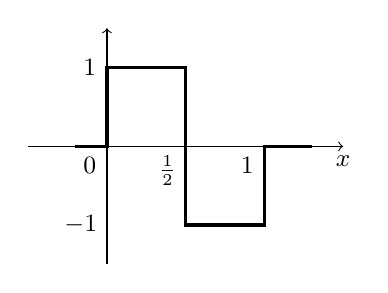
\begin{tikzpicture}[xscale=2]
      \draw [thin,->] (0,-1.5) -- (0,1.5);
      \draw [thin,->] (-0.5,0) -- (1.5,0) node[below]{\small$x$};
      \draw [very thick] (-0.2,0) -- (0,0) node[below left]{\small$0$} -- (0,1) node[left]{\small $1$} -- (0.5,1) -- (0.5,-1) -- (1,-1) -- (1,0) node[below left]{\small $1$} -- (1.3,0);
      \node at (0,-1)[left]{\small$-1$};
      \node at (0.5,0)[below left]{\small $\frac{1}{2}$};
    \end{tikzpicture}
    \caption{Haar mother wavelet $\psi(x)$}
    \label{fig:haar_mother}
  \end{subfigure}
  \caption{The scaling function and wavelet function for the Haar wavelets.}
  \label{fig:haar_1d}
\end{figure}

For example, for the \emph{Haar wavelets} the scaling function is given by
\begin{equation}
  \label{eqn:haar_scale}
  \phi(x) = \left\{ \begin{array}{rl}
    1& \qquad \mbox{if $0\leq x < 1$}\\
    0& \qquad \mbox{otherwise}
  \end{array}\right.
\end{equation}
See Figure \ref{fig:haar_scaling} for a plot of $\phi(x)$.

Given the scaling function $\phi(x)$, we can define the following basis for $V^j$:
\begin{equation*}
  \phi_k^j(x) := 2^{j/2}\phi(2^j x-k) \qquad k = 0,\cdots, 2^j-1
\end{equation*}

Using this basis, we can decompose our signal $v(x)\in V^q$ as 
\begin{equation*}
  v(x) = \sum_{k=0}^{2^q-1} c_k^q \phi_k^q(x)
\end{equation*}
For the scaling function defined in equation (\ref{eqn:haar_scale}), we have that $c_k^q = v_{k+1}$.

To obtain \emph{wavelets}, consider the \emph{orthogonal complement} of $V^j$ in $V^{j+1}$ and denote it $W^j$. 
That is, $W^j = \{f \in V^{j+1} :\quad \langle f,g\rangle = 0\quad \forall g \in V^j\}$ where the inner product $\langle f,g\rangle$ is given by
\begin{equation*}
  \langle f,g\rangle = \int_0^1f(x)g(x)dx.
\end{equation*}
By forming a basis for $W^j$, we obtain a set of \emph{wavelet functions} $\{\psi_k^j,\, k=0,\cdots,2^j-1\}$.
Wavelet functions can be constructed by scaling and shifting a so-called \emph{mother wavelet} $\psi(x)$ as follows:
\begin{equation*}
  \psi_k^j(x) = 2^{j/2}\psi(2^j x - k) \qquad k = 0,\cdots, 2^j-1
\end{equation*}

For the Haar wavelets, the mother wavelet is given by:
\begin{equation}
\label{eqn:haar_mother}
  \psi(x) = \left\{\begin{array}{rl}
  1&\qquad 0 \leq x < 1/2\\
  -1&\qquad 1/2 \leq x < 1\\
  0&\qquad\mbox{otherwise}
  \end{array}\right.
\end{equation}
The Haar mother wavelet is shown in Figure \ref{fig:haar_mother}.

Note that, since the scaling functions $\phi_k^j$ form a basis of $V^j$ and the wavelet functions $\psi_k^j$ form a basis of $W^k$, and since $W^j$ is the orthogonal complement to $V^j$ in $V^{j+1}$, it follows that the set $\{\phi_k^j, \psi_k^j: k=0,\cdots,2^j-1\}$ forms a basis of the vector space $V^{j+1}$.

This allows us to express our signal $v \in V^q$ as 
\begin{equation*}
  v(x) = \sum_{k=0}^{2^{q-1}-1} d_k^{q-1}\psi_k^{q-1}(x) + \sum_{k=0}^{2^{q-1}-1} c_k^{q-1}\phi_k^{q-1}(x)
\end{equation*}
This gives us the first level of the discrete wavelet transform of $v$.
The coefficients $c_k$ and $d_k$ are sometimes referred to as ``approximation'' coefficients and ``detail'' coefficients, respectively.

We can continue the decomposition by splitting the basis for $V^{q-1}$ into the bases for $V^{q-2}$ and $W^{q-2}$ to get the next level of the transform:
\begin{equation*}
  v(x) = \sum_{k=0}^{2^{q-1}-1} d_k^{q-1}\psi_k^{q-1}(x) + \sum_{k=0}^{2^{q-2}-1} d_k^{q-2}\psi_k^{q-2}(x) + \sum_{k=0}^{2^{q-2}-1} c_k^{q-2}\phi_k^{q-2}(x)
\end{equation*}
To get the full decomposition, we continue in this fashion up to the $q$th level:
\begin{equation*}
  v(x) = \sum_{j=0}^{q-1} \sum_{k=0}^{2^j-1} d_k^{j} \psi_k^j(x) + c_0^0\phi(x)
\end{equation*}
The full DWT of $\bm v$ consists of the coefficients $\{c_0^0, d_k^j:\,j=0,\cdots,q-1, \, k=0,\cdots,2^j-1\}$.


\subsection{Computing the DWT}

\begin{figure}
  \centering
  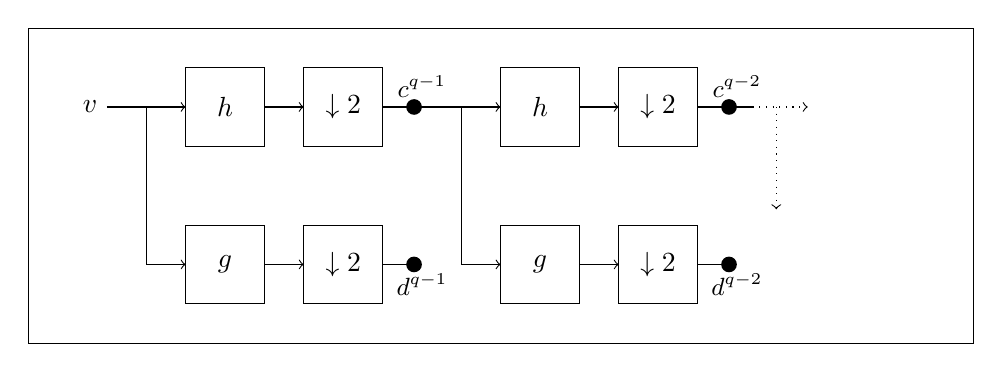
\begin{tikzpicture}
    \draw (0,0) rectangle (12,4);
    \draw (1,3) node[left]{$v$} -- (1.5,3);
    \draw (1.5,1) -- (1.5,3);
    \draw [->](1.5,3) -- (2,3);
    \draw [->](1.5,1) -- (2,1);
    \draw (2,2.5) rectangle (3,3.5);
    \node at (2.5,3) {$h$};
    \draw (2,0.5) rectangle (3,1.5);
    \node at (2.5,1) {$g$};
    \draw [->](3,1) -- (3.5,1);
    \draw (3.5,0.5) rectangle (4.5,1.5);
    \node at (4,1) {$\downarrow 2$};
    \draw (4.5,1) -- (5,1) node [below] {\small$d^{q-1}$};
    \node at (4.9,1)[shape=circle, fill=black, inner sep=2pt, minimum size=2pt] {};
    \draw [->](3,3) -- (3.5,3);
    \draw (3.5,2.5) rectangle (4.5,3.5);
    \node at (4,3) {$\downarrow 2$};
    \draw [->](4.5,3) -- (6,3);
    \draw [->](5.5,3) -- (5.5,1) -- (6,1);
    \node at (5,3) [above] {\small$c^{q-1}$};
    \node at (4.9,3) [shape=circle, fill=black, inner sep=2pt, minimum size=2pt] {};
    \draw (6,2.5) rectangle (7,3.5);
    \node at (6.5,3){$h$};
    \draw (6,0.5) rectangle (7,1.5);    
    \node at (6.5,1){$g$};
    \draw [->] (7,3) -- (7.5,3);
    \draw (7.5,2.5) rectangle (8.5,3.5);
    \node at (8,3) {$\downarrow 2$};
    \draw [->] (7,1) -- (7.5,1);
    \draw (7.5,0.5) rectangle (8.5,1.5);
    \node at (8,1) {$\downarrow 2$};
    \draw (8.5,1) -- (9,1) node [below] {\small$d^{q-2}$};
    \node at (8.9,1) [shape=circle, fill=black, inner sep=2pt, minimum size=2pt] {};
    \draw (8.5,3) -- (9.2,3);
    \draw [->,dotted](9.2,3) -- (9.9,3);
    \draw [->,dotted](9.5,3) -- (9.5,1.7);
    \node at (8.9,3) [shape=circle, fill=black, inner sep=2pt, minimum size=2pt] {};
    \node at (9,3) [above] {\small$c^{q-2}$};
  \end{tikzpicture}
  \caption{The first two levels of the DWT of the signal $\bm v$ of length $2^q$ via a filter bank.}
  \label{fig:filterbank}
\end{figure}

In practice, we can compute one level of the DWT coefficients by passing the signal $v$ through a \emph{low-pass filter} $h$ and a high-pass filter $g$, respectively, and then downsampling the results by a factor of two.
Passing $v$ through the filters $h$ and $g$ results in the \emph{convolutions}:
\begin{equation*}
  \begin{split}
    (v\star h)(x) &= \sum_{k=-\infty}^\infty v(k)h(x-k)\\
    (v\star g)(x) &= \sum_{k=-\infty}^\infty v(k)g(x-k)
  \end{split}
\end{equation*}
To downsample by a factor of two, we remove every second sample:
\begin{equation*}
  (v\downarrow 2)(x) := v(2x)
\end{equation*}

Overall, these computations can be done by multiplying the vector $\bm v$ by a matrix $\bm H$ and a matrix $\bm G$ to get the approximation and detail coefficients, repectively.

To compute the next level, we take the approximation coefficients of the current stage and pass them again through the filter bank.
The procedure is depicted in Figure \ref{fig:filterbank}.

The coefficients of the filters $h(x)$ and $g(x)$ depend on our choice of the scaling function $\phi(x)$ and mother wavelet function $\psi(x)$.
They satisfy the following relations:
\begin{equation*}
  \begin{split}
    \phi(x) &= \sqrt{2}\sum_{k=-\infty}^\infty h(k)\phi(2x - k)\\
    \psi(x) &= \sqrt{2}\sum_{k=-\infty}^\infty g(k)\phi(2x - k)
  \end{split}
\end{equation*}
as well as
\begin{equation*}
  g(k) = (-1)^k h(1-k).
\end{equation*}

For the Haar wavelets (\ref{eqn:haar_scale},\ref{eqn:haar_mother}), the filter coefficients are
\begin{equation*}
  \begin{split}
    h(0) = h(1) &= \frac{1}{\sqrt{2}}\\
    g(0) = -g(1) &= \frac{1}{\sqrt{2}}
  \end{split}
\end{equation*}




%% The simplest wavelet basis transformation is based on the Haar wavelets.
%% Figure \ref{fig:haarlenna} vizualises a basis transformation of the original image $\bs x$ to $\bs w$. 
%% This example uses a Haar wavelet basis at the first scale.
%% We will explain the Haar wavelet transformations of images and videos in more detail in the next chapter.
%% Dark areas correspond to small coefficients.
%% Note that most entries in $\bs w$ are near zero. 
%% In practice, we approximate these entries as zero and treat $\bs w$ as sparse.

%% \begin{figure}
%% \center
%% 
\includegraphics{Images/128.png}
%% 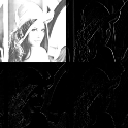
\includegraphics{Images/haar.png}
%% \caption{Original image $\bs x$ (left) and its Haar basis transformation $\bs w$ (right). See next chapter for more details on Haar wavelets.}
%% \label{fig:haarlenna}
%% \end{figure}

%% \section{Haar basis functions}
%% The RVM takes as input a target vector ($\bs y$) and a basis matrix ($\bs \Psi$). 
%% In this respect, it is agnostic about whether the signal is an image or video or of some other type alltogether.
%% Most of this information is encoded in the basis matrix $\bs \Psi$.
%% It is therefore important, and often challenging, to select a good set of basis functions.

%% Our current implementation uses 3-dimensional Haar wavelet basis functions.
%% I will show how the basis matrix $\bs\Psi$ is constructed by briefly describing how the discrete Haar wavelet transform is performed on 1D, 2D and finally on 3D signals.
%% \subsection{1D Haar wavelet transform}
%% Consider a 1-dimensional signal $\bs s = \{s_1,\dots,s_r\} \in \mathbb{R}^r$ ($r$ for ``rows''), where, for simplicity, we assume that $r$ is a power of 2.
%% The Haar wavelet transform can be performed at various resolution scales.
%% The transform at the first scale is given by:
%% \begin{equation*}
%% \bs s = \{s_1,\dots,s_r\}\to \frac{1}{\sqrt{2}}\{s_1+s_2,s_3+s_4,\dots,s_{r-1}+s_r,s_1-s_2,\dots,s_{r-1}-s_r\}=\hat{\bs s}^{(1)}
%% \end{equation*}
%% The first half of the signal is replaced by scaled averages of adjacent elements and the second half is replaced by scaled differences of adjacent elements.
%% By performing this transform again on the first half of $\hat{\bs s}^{(1)}$ while keeping the second half fixed, we get the Haar wavelet transform at the second scale $\hat{\bs s}^{(2)}$. 
%% To get the third scale transform $\hat{\bs s}^{(3)}$, we perform the initial transform on the first quarter of $\hat{\bs s}^{(2)}$ while keeping the rest of the signal fixed.
%% We may continue this process until we reach the $i$th scale, where $2^i = r$.

%% From here on, we will only consider the first scale transform $\hat{\bs s}^{(1)}$ and we will omit the $(1)$ superscript.
%% We can express the transform as a multiplication by an orthogonal $r\times r$ matrix $W$ given by
%% \begin{equation}
%% W = \begin{bmatrix}
%%   \Phi_r \\
%%   \Psi_r \\
%% \end{bmatrix}
%% \end{equation}
%% where $\Phi_r$ and $\Psi_r$ are $(r/2)\times r$ matrices\footnote{Note that the matrix $\Psi_r$ used here is different to the matrix $\Psi$ that was used in the previous chapter (which corresponds to $W^T$ here).} given by
%% \begin{equation*}
%% \Phi_r = \frac{1}{\sqrt{2}} \begin{pmatrix}
%% 1&1&0&0&\cdots&0&0\\
%% 0&0&1&1&\cdots&0&0\\
%% \vdots&\vdots&\vdots&\vdots&\ddots&\vdots&\vdots\\
%% 0&0&0&0&\cdots&1&1
%% \end{pmatrix}
%% \end{equation*}
%% and 
%% \begin{equation*}
%% \Psi_r = \frac{1}{\sqrt{2}} \begin{pmatrix}
%% 1&-1&0&0&\cdots&0&0\\
%% 0&0&1&-1&\cdots&0&0\\
%% \vdots&\vdots&\vdots&\vdots&\ddots&\vdots&\vdots\\
%% 0&0&0&0&\cdots&1&-1
%% \end{pmatrix}
%% \end{equation*}


%% In the signal processing literature, $\Phi_r$ is referred to as a low pass filter, while $\Psi_r$ is referred to as a high pass filter.
%% $\Phi_r$ outputs an average of the signal and $\Psi_r$ outputs the details of the signal.

%% \subsection{2D Haar wavelet transform}
%% Let $A \in \mathbb{R}^{r\times c}$ be a 2-dimensional signal (e.g. an image).
%% For simplicity, we will assume that both $r$ and $c$ are powers of 2 (though not necessarily equal).

%% It is simple to obtain $A$'s Haar wavelet transform $\hat{A}$ at the first scale.
%% This is done by first applying the 1-dimensional transform individually to each column of $A$ to obtain a temporary matrix $\hat A_{temp}$.
%% Next, we apply the 1-dimensional haar wavelet transform individually to each row of $\hat A_{temp}$ to obtain $\hat A$.

%% We can again express the transform as a multiplication of matrices:
%% \begin{equation}
%% \label{eqn:2Dtransform}
%% \hat A = \begin{bmatrix}
%%   \Phi_r\\
%%   \Psi_r\\
%% \end{bmatrix}
%% A
%% \begin{bmatrix}
%%   \Phi_c^T & \Psi_c^T\\
%% \end{bmatrix}
%% \end{equation}
%% where $\Phi_r$ and $\Psi_r$ are as before and $\Phi_c$ and $\Psi_c$ are of similar form but each have dimensions $(c/2)\times c$.
%% This is the transform that was used to generate the RHS of Figure \ref{fig:haarlenna}.
%% We note that the high-pass filters essentially detect edges of various orientations in the image.

%% However, as it currently stands, we cannot use this form of the basis transformation for the reconstruction algorithm. Recall that the RVM requires a \emph{vector} of measurements as opposed to a matrix and also that it requires a single basis matrix, not a basis transform as given in (\ref{eqn:2Dtransform}).

%% To do this, we store the 2-dimensional signal $A$ as a long column vector $\bs a$ of length $rc$ by pasting the individual columns of $A$ one after another.
%% The basis transformation of $\bs a$ can then be expressed as 
%% \begin{equation*}
%% \hat{\bs a} = W \bs a
%% \end{equation*}
%% where $W$ is a $rc \times rc $ matrix given by
%% \begin{equation*}
%% W = 
%% \begin{bmatrix}
%% \Phi_c \otimes \Phi_r \\
%% \Phi_c \otimes \Psi_r \\
%% \Psi_c \otimes \Phi_r \\
%% \Psi_c \otimes \Psi_r \\
%% \end{bmatrix}
%% \end{equation*}

%% The symbol $\otimes$ denotes the \emph{Kronecker product}. 
%% The kronecker product $P \otimes Q$ between matrices $P$ and $Q$ with dimensions $m_P \times n_P$ and $m_Q \times n_Q$, respectively,  is defined to be the block matrix
%% \begin{equation*}
%% \begin{bmatrix}
%% p_{1,1} Q & p_{1,2} Q & \cdots & p_{1,n_P} Q \\
%% p_{2,1} Q & p_{2,2} Q & \cdots & p_{2,n_P} Q \\
%% \vdots&\vdots&\ddots&\vdots \\
%% p_{m_P,1} Q & p_{m_P,2} Q & \cdots & p_{m_P,n_P} Q \\
%% \end{bmatrix}
%% \end{equation*}
%% of size $m_Pm_Q \times n_Pn_Q$.

%% \subsection{3D Haar wavelet transform}
%% Let $V \in \mathbb{R}^{r\times c\times s}$ be a 3-dimensional signal such as a video. 
%% $V$ has $r$ rows, $c$ columns and $s$ slices, and we assume that $r$, $c$ and $s$ are all powers of 2. 
%% We may visualize $V$ as a ``volume'' with 2 spacial dimensions and one time dimension corresponding to frames of the video.

%% To obtain the Haar wavelet transform $\hat V$ of $V$, we first perform the 1-dimensional transform individually on each column in every slice of $V$ to get $\hat V_{temp1}$.
%% We then perform the 1D transform on every row in every slice of $\hat V_{temp_1}$ to get $\hat V_{temp_2}$.
%% Finally, we perform the 1D transform across the slices for every row and column to get $\hat V$.

%% However, like in the 2-dimensional case, we need to be able to pass a single vector of coefficients and a single basis matrix to the RVM.
%% To do this, we vectorize $V$ as follows. 
%% First, we vectorize each individual slice of $V$ as before in the 2D case.
%% Then, we stack all these vectors on top each other to get one very long column vector $\bs v$ of length $rcs$.
%% The Haar wavelet transform is given by 
%% \begin{equation*}
%% \hat{\bs v} = W \bs v
%% \end{equation*}
%% where 
%% \begin{equation*}
%% W = 
%% \begin{bmatrix}
%% \Phi_s \otimes \Phi_c \otimes \Phi_r \\
%% \Phi_s \otimes \Phi_c \otimes \Psi_r \\
%% \Phi_s \otimes \Psi_c \otimes \Phi_r \\
%% \Phi_s \otimes \Psi_c \otimes \Psi_r \\
%% \Psi_s \otimes \Phi_c \otimes \Phi_r \\
%% \Psi_s \otimes \Phi_c \otimes \Psi_r \\
%% \Psi_s \otimes \Psi_c \otimes \Phi_r \\
%% \Psi_s \otimes \Psi_c \otimes \Psi_r \\
%% \end{bmatrix}
%% \end{equation*}


%% \subsection{Daubechies Wavelets}
%% \emph{Intuition. Where do the coeffs come from. Matrices. Boundary conditions.}


%% \section{Forming the basis matrix}
%% \emph{1D, 2D, 3D case. Different scales}

%% For a deeper introduction into wavelets see \cite{stollnitz1995}.
%% For more information on wavelet compression techniques, see \cite{devore1992}.



